\documentclass{scrreprt}
\usepackage[english]{babel}
\usepackage[T1]{fontenc}
\usepackage{lmodern}
\usepackage{blindtext}
\usepackage[utf8]{inputenc}
\usepackage{siunitx} %For unit handling%
\renewcommand{\familydefault}{\sfdefault}
\newcommand{\unit}[1]{\ensuremath{\, \mathrm{#1}}}
\usepackage{amssymb, amsmath, cancel, ulem, graphicx, float, tabularx, multirow, bm}
\usepackage{amsmath}

\setcounter{secnumdepth}{5}
\setcounter{tocdepth}{5}

\renewcommand{\emph}[1]{\textit{#1}}

\author{Urs Gerber\\09-921-156 \and Gian-Luca Mateo\\11-113-545}
\date{14th of March 2013}

\title{Collision Experiment}
\subtitle{Practical course report}

\begin{document}

\maketitle

\tableofcontents
\newpage

\chapter{Experiment: Momentum Conservation}
\section{Introduction}
A collision is a short-time interaction between two or more objects. In essence there are two types of collisions: the \emph{elastic} collision and the \emph{inelastic} collision.\\
In an ideal elastic collision no energy is lost during the course of the interaction, meaning no energy is lost due to heat or deformation. 
 
\subsection{Goal of the experiment}
\subsection{Theory}
\subsubsection{Preliminary exercises}
Using $A:=\frac{m_2}{m_1}$

\paragraph*{Task 1}
\begin{equation}
m_1v_1=m_1v_1'+m_2v_2'
\end{equation}
\begin{equation}
\Rightarrow v_2'=\frac{m_1}{m_2}(v_1-v_1')
\end{equation}
\begin{equation}
\frac{1}{2}m_1v_1^2=\frac{1}{2}m_1v_1'^2+\frac{1}{2}m_2v_2'^2
\end{equation}
\begin{equation}
\Rightarrow m_1v_1^2=m_1v_1'^2+\frac{m_1^2}{m_2}(v_1-v_1')^2
\end{equation}
\begin{equation}
\Rightarrow v_1^2=v_1'^2+\frac{m_1}{m_2}(v_1-v_1')^2
\end{equation}
\begin{equation}
\Rightarrow v_1^2-v_1^2=\frac{m_1}{m_2}(v_1-v_1')^2
\end{equation}
\begin{equation}
\Rightarrow (v_1+v_1')=\frac{m_1}{m_2}(v_1-v_1')
\end{equation}
\begin{equation}
\Rightarrow v_1+v_1'=\frac{1}{A}(v_1-v_1')
\end{equation}
\begin{equation}
\Rightarrow v_1-\frac{v_1}{A}=-v_1-\frac{v_1'}{A}
\end{equation}
\begin{equation}
\Rightarrow v_1\left(1-\frac{1}{A}\right)=-v_1'\left(1+\frac{1}{A}\right)
\end{equation}
\begin{equation}
\Rightarrow \frac{v_1'}{v_1}=-\frac{1-\frac{1}{A}}{1+\frac{1}{A}} = \frac{A-1}{-A-1}
\end{equation}
\begin{equation}
\Rightarrow \frac{T_1'}{T_1} = \left(\frac{A-1}{-(A+1)}\right)^2=\left(\frac{A-1}{A+1}\right)^2
\end{equation}

\paragraph*{Task 2}
\begin{equation}
\frac{T_{1,2}'}{T_1}=\frac{(m_1+m_2)v_1'^2}{m_1v_1^2}
\end{equation}
\begin{equation}
v_1'=v_1\frac{m_1}{m_1+m_2}
\end{equation}
\begin{equation}
\Rightarrow \frac{T_1'}{T_1}= \frac{(m_1+m_2)}{m_1}\frac{v_1^2\left(\frac{m_1}{m_1+m_2}\right)^2}{v_1^2}=\frac{m_1}{m_1+m_2}=\frac{1}{1+A}
\end{equation}
\begin{equation}
\Rightarrow \frac{Q}{T_1}=1-\frac{T_1'}{T_1}=1-\frac{1}{1+A}=\frac{A}{1+A}
\end{equation}
Q is the fraction of the energy of $T_1$ lost in the collision. Q is composed of thermic energy, deformation energy and sound.

\paragraph*{Task 3}
\begin{equation}
l^2=a^2+(l-h)^2=a^2+l^2-2lh+\underbrace{h^2}_{\approx 0}
\end{equation}
\begin{equation}
\Rightarrow h=\frac{a^2}{2l}
\end{equation}
\begin{equation}
\frac{1}{2}m_2v_2'^2=m_2gh_2 \mbox{ und } \frac{1}{2}m_1v_1^2=m_1gh_1
\end{equation}
\begin{equation}
\frac{T_2'}{T_1}=\frac{m_2gh_2}{m_1gh_1}=\frac{m_2\frac{a_2^2}{2l}}{m_1\frac{a_1^2}{2l}}=\frac{m_2a_2^2}{m_1a_1^2}=A\frac{a_2^2}{a_1^2}
\end{equation}

\paragraph*{Task 4}
\begin{figure}[H]
	\centering
  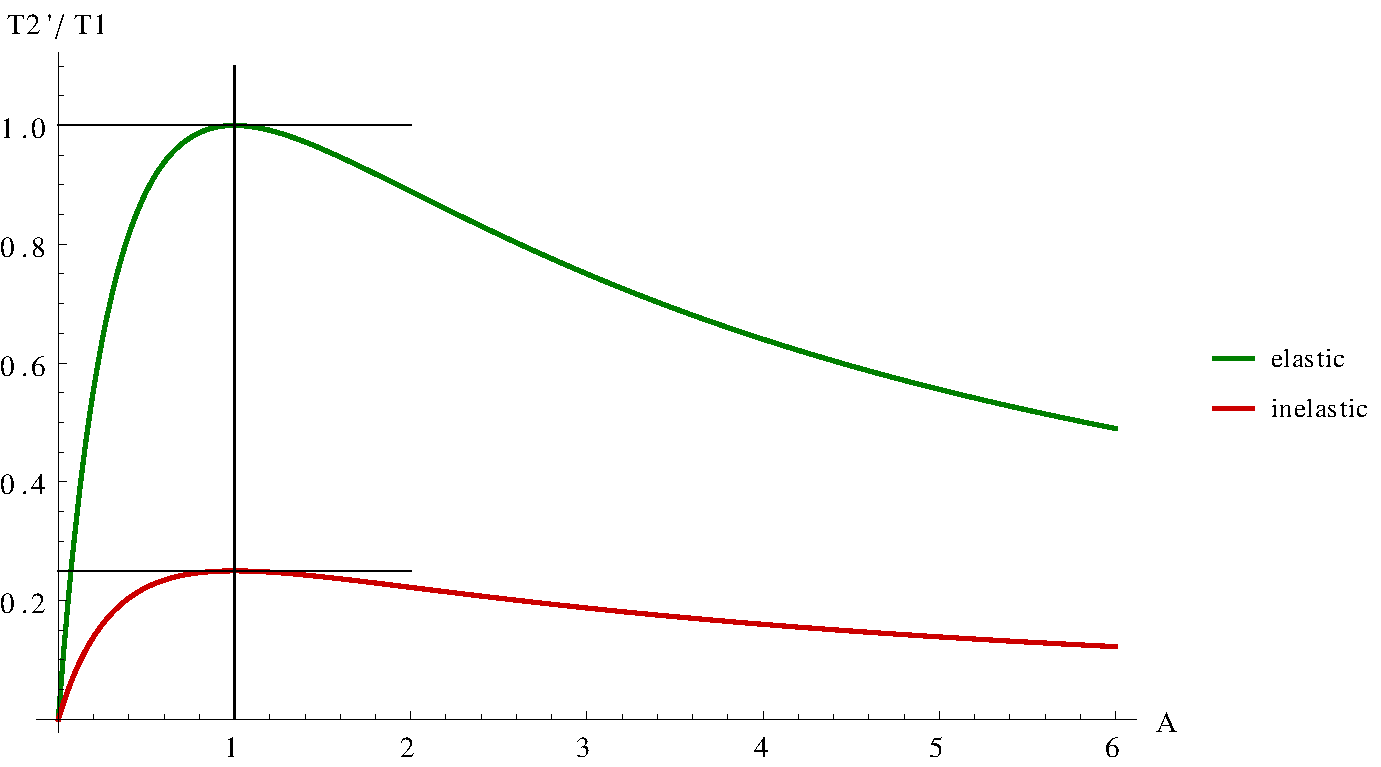
\includegraphics[width=0.9\textwidth]{diag/collision.pdf}
	\caption{$T_2'/T_1$ in dependance of $A$}
	\label{fig:task4}
\end{figure}
\noindent Figure \ref{fig:task4} shows the progression of $T_2'/T_1$ dependance of $A$ for an elastic and inelastic collision.\\
One can easily see that the maximum transfer of energy occurs at $A=1\Leftrightarrow m_1=m_2$

\paragraph*{Task 5}
We need the following formulae to analyze our data:
\begin{center}
\begin{tabular}{lrl}
Theory, elastic & $T_2'/T_1 = $ &  $\frac{4A}{(A+1)^2}$ \\
Theory, inelastic &$T_2'/T_1 =$ &  $\frac{A}{(A+1)^2}$ \\
Measurment & $T_2'/T_1 = $ & $A \frac{a_2^2}{a_1^2}$ \\
Theory & $Q/T_1 = $ & $\frac{A}{1+A}$ \\
Measurement & $Q/T_1 =$ & $1-(1+A)\frac{a_2^2}{a_1^2}$ \\
\end{tabular}
\end{center}

\section{Experiment setup and execution}

\subsection{Used materials}
\begin{figure}[H]
	\centering
  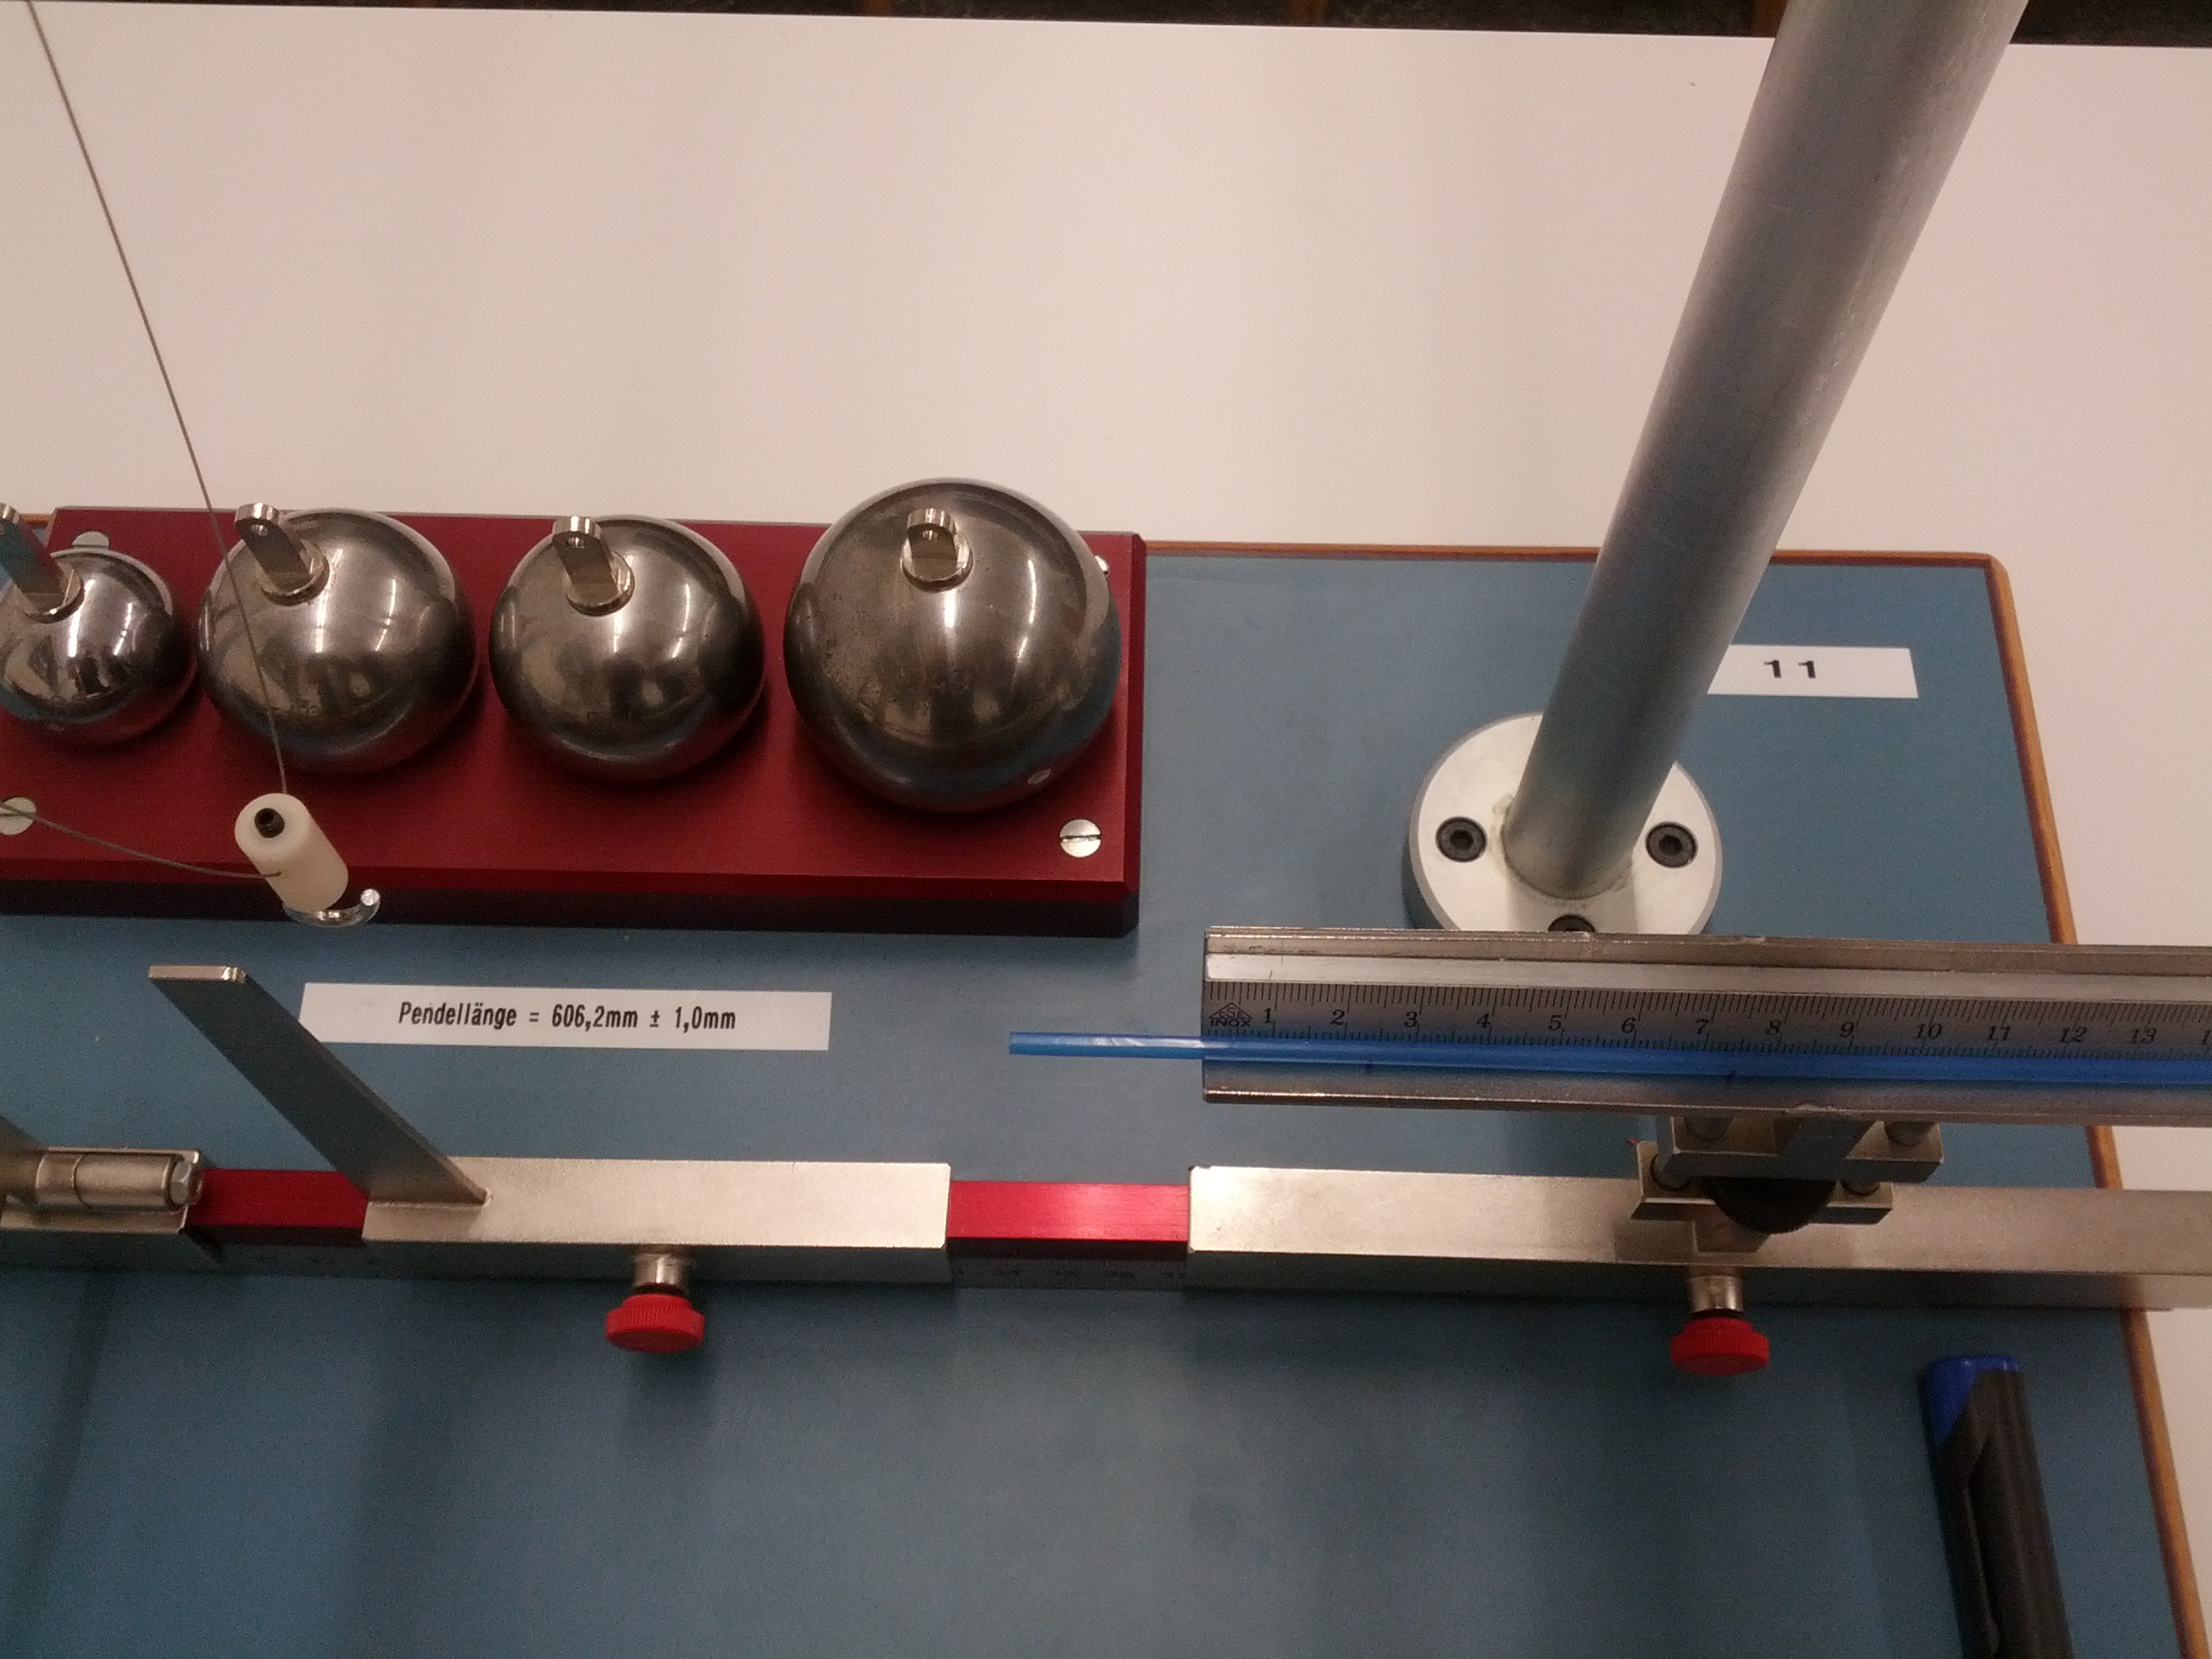
\includegraphics[width=0.9\textwidth]{img/topview.jpg}
	\caption{All used materials}
	\label{fig:materials}
\end{figure}

\subsection{Assembly}
\begin{figure}[H]
	\centering
  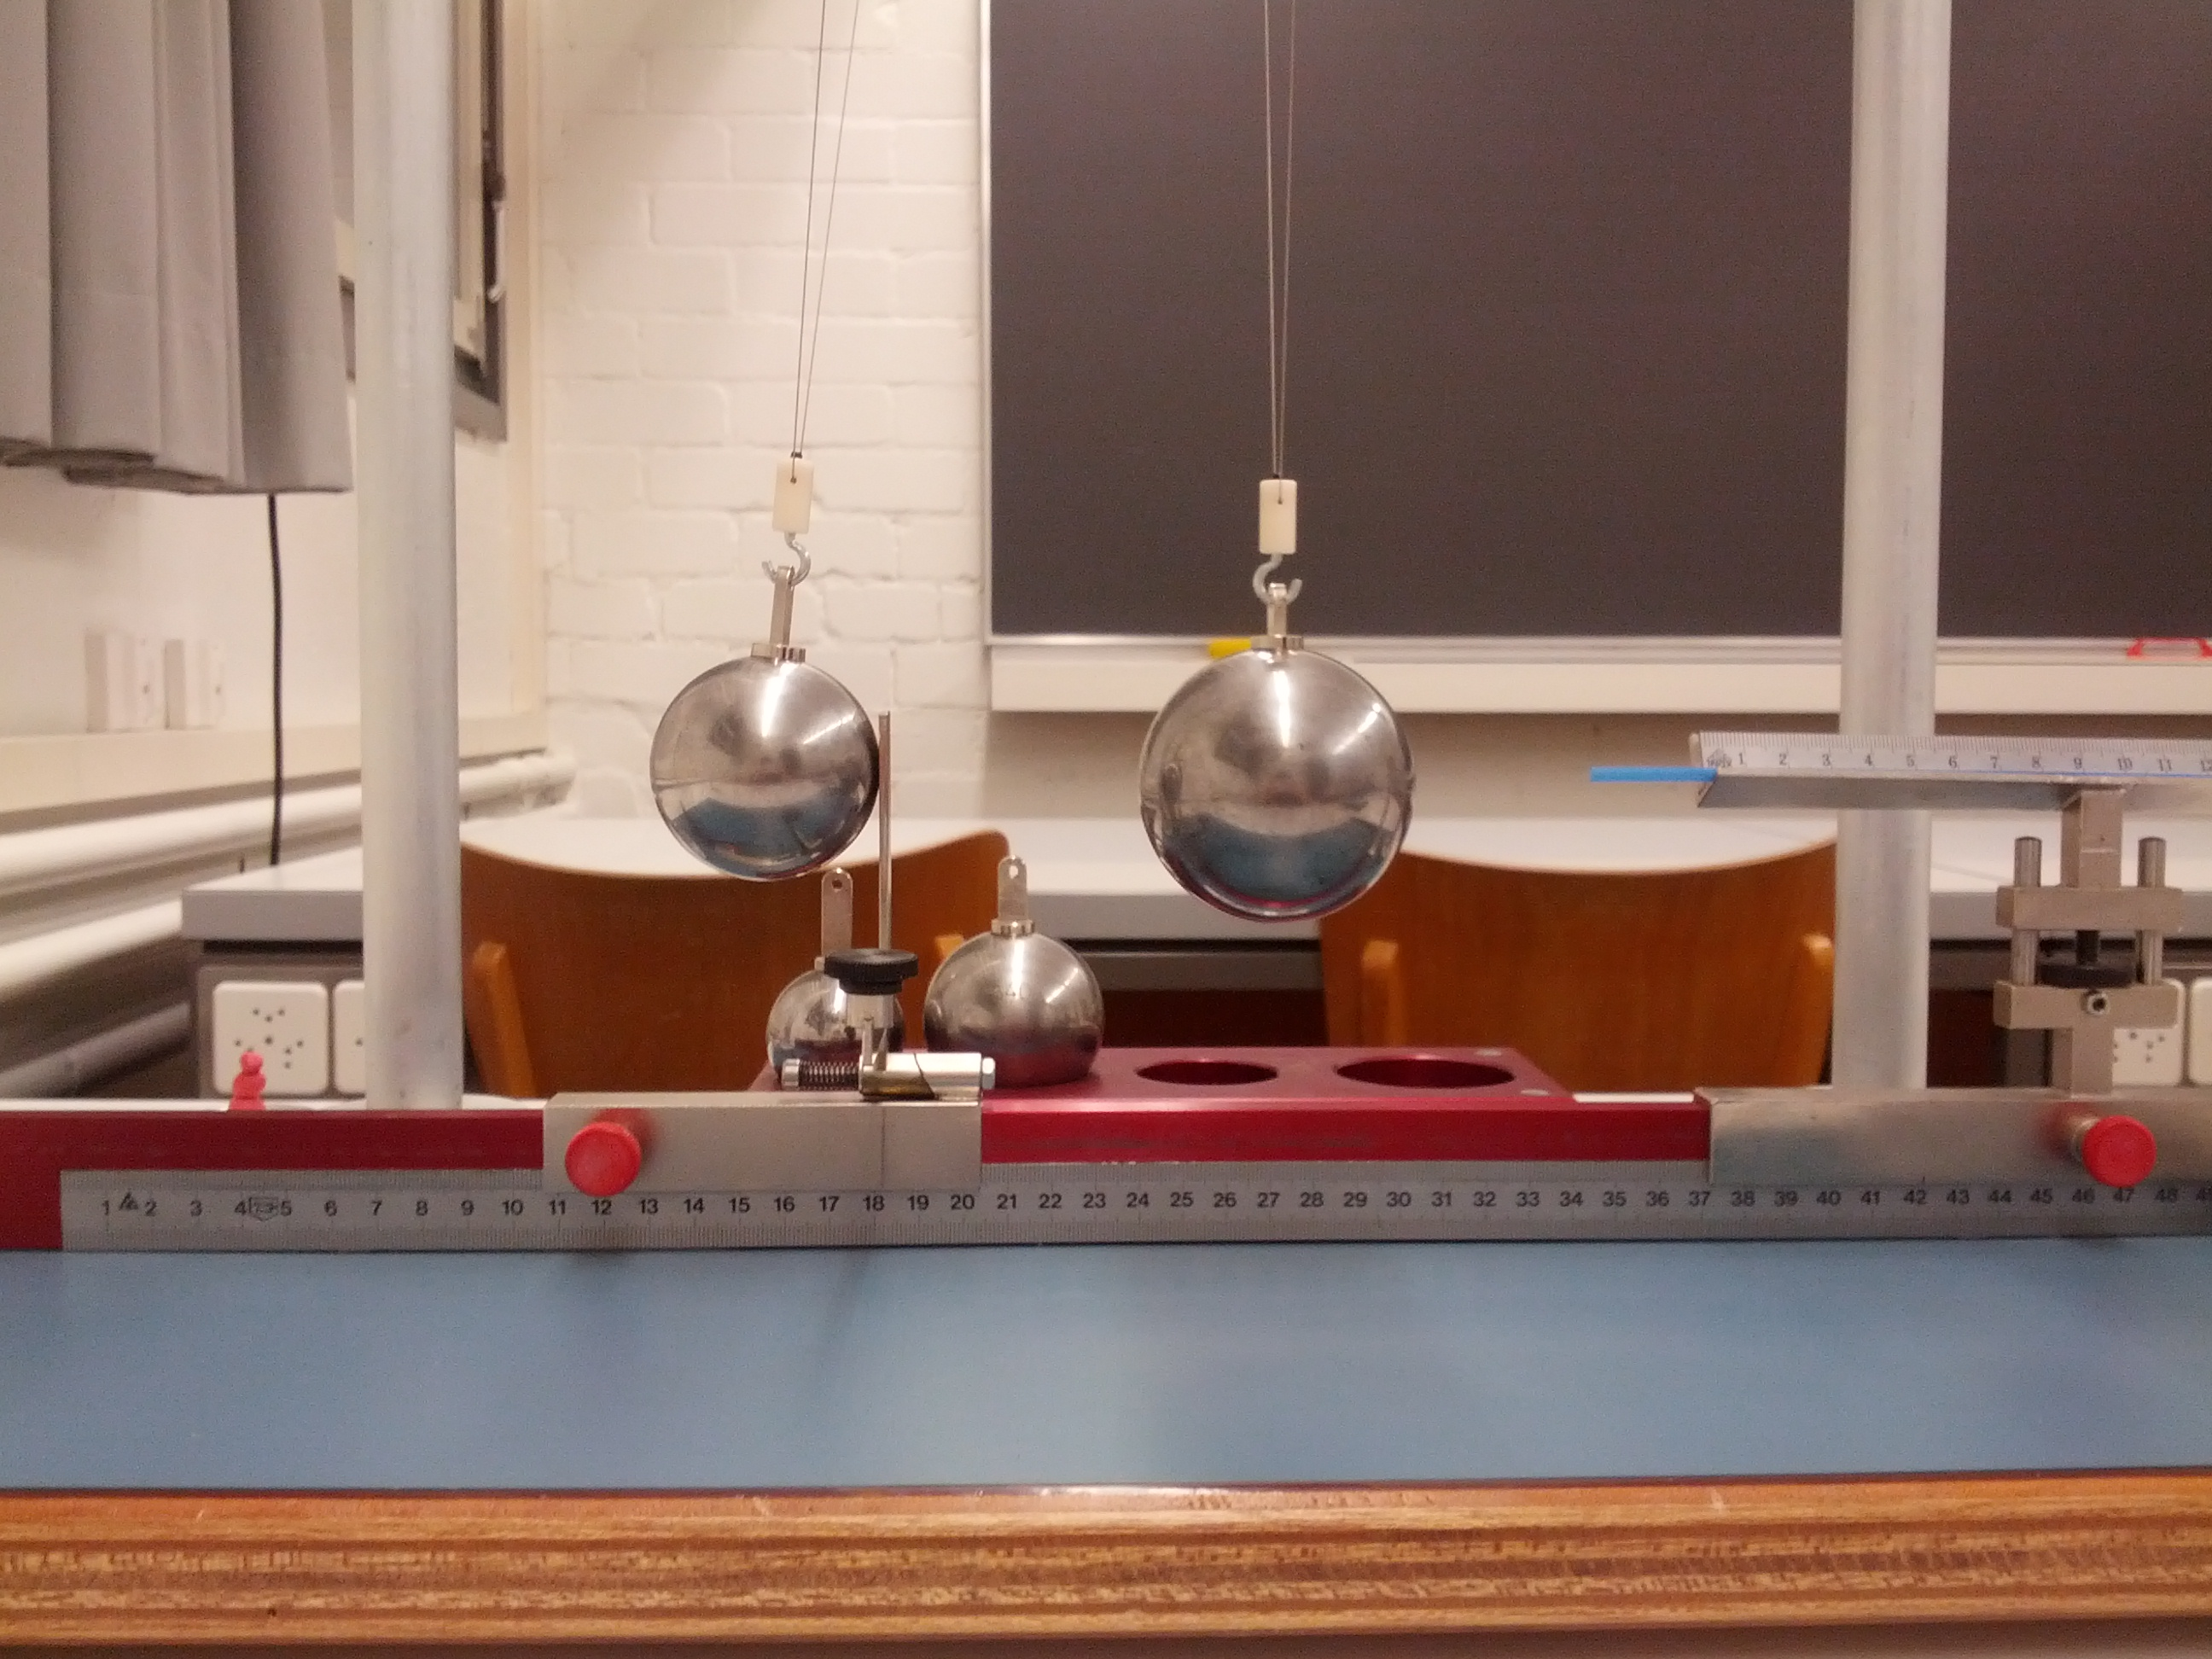
\includegraphics[width=0.9\textwidth]{img/assembly.jpg}
	\caption{Final experiment assembly}
	\label{fig:assembly}
\end{figure}

\section{Measurements and analysis}
\section{Discussion}


\begin{thebibliography}{9}

\bibitem{physcript13}
  Peter Wurz,
  \emph{Anleitung zum Physikpraktikum}
  FS2013

\end{thebibliography}

\end{document}
